\documentclass[12pt]{article}

\usepackage{bm}
\usepackage{amsmath}
\usepackage{amssymb}
\usepackage{cite}
\usepackage{indentfirst}
\usepackage{url}
\usepackage{graphicx}

\title{Project 2 \\\vspace{1em}
\large CS 525: Deep Learning}
\author{
  Jerry Duncan \\
  jdunca51@vols.utk.edu
}
\date{February 23, 2020}
\begin{document}
\maketitle
\pagebreak

\section{Introduction}

For this project, we're extending our previous project to now work on image-like data.
More specifically, we've added Convolutional, Flatten, and Max Pooling layers so that we can create a Convolutional Neural Network.
This means that we're not able to solve a larger range of problems with our library than when it was just a Fully Connected Neural Network.
We can now tackle image data as well as unique problems that benefit from convolving over the input.

\section{Assumptions / Choices Made}

The only differences from the stated requirements and my code is as follows:
\begin{itemize}
  \item My addLayer function has been renamed add
  \item The shape of my weights has been finagled to match those of Keras
\end{itemize}

\section{Problems / Issues}

Nothing to add.

\section{Running My Code}

Run ``python main.py $<$example\#$>$''. That's the driver file, the rest is the library.

\section{Weight Comparison}

In Figure \ref{fig:e1}, \ref{fig:e2}, and \ref{fig:e3} are my weight comparisons.
On the left is the weights before backprop, showing that they've been set to be equal between both models.
The right is after backprop to show they're still the same, except for some small rounding errors between when and where the two models truncate their values.
This also helps show that my model is my own code since they're not quite exactly equal.
 This is especially noticeable in the biases).

\begin{figure}
  \centering
  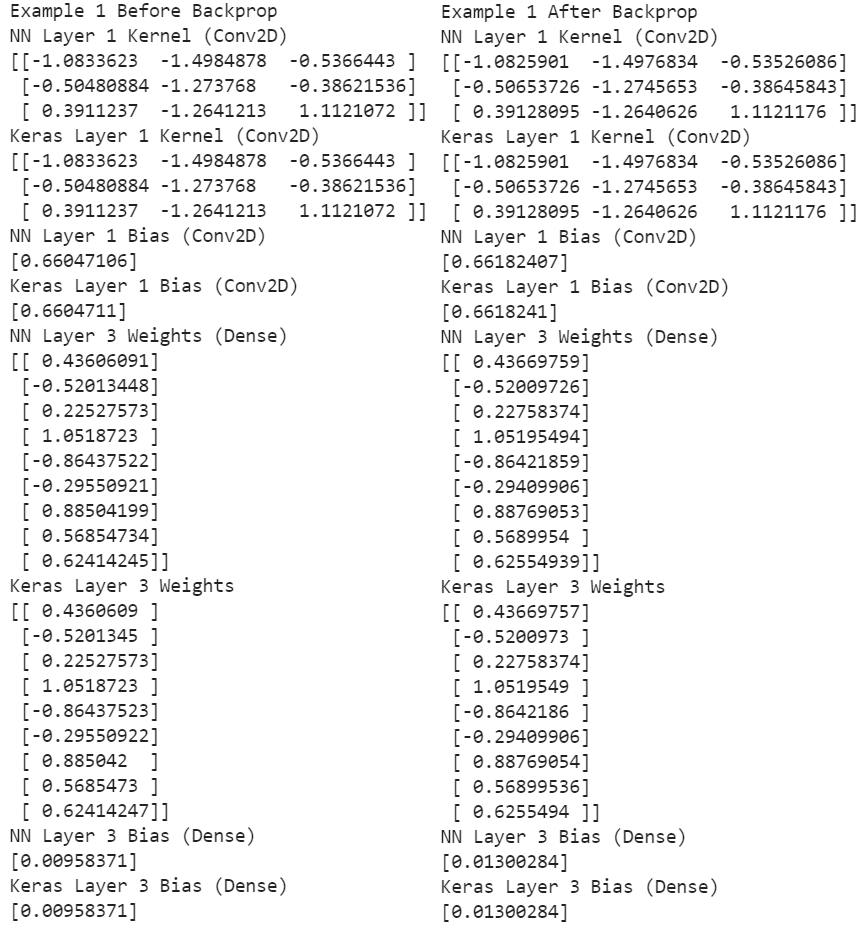
\includegraphics[width=\linewidth]{example-1-weights.png}
  \caption{Weight comparison for example 1.}
  \label{fig:e1}
\end{figure}

\begin{figure}
  \centering
  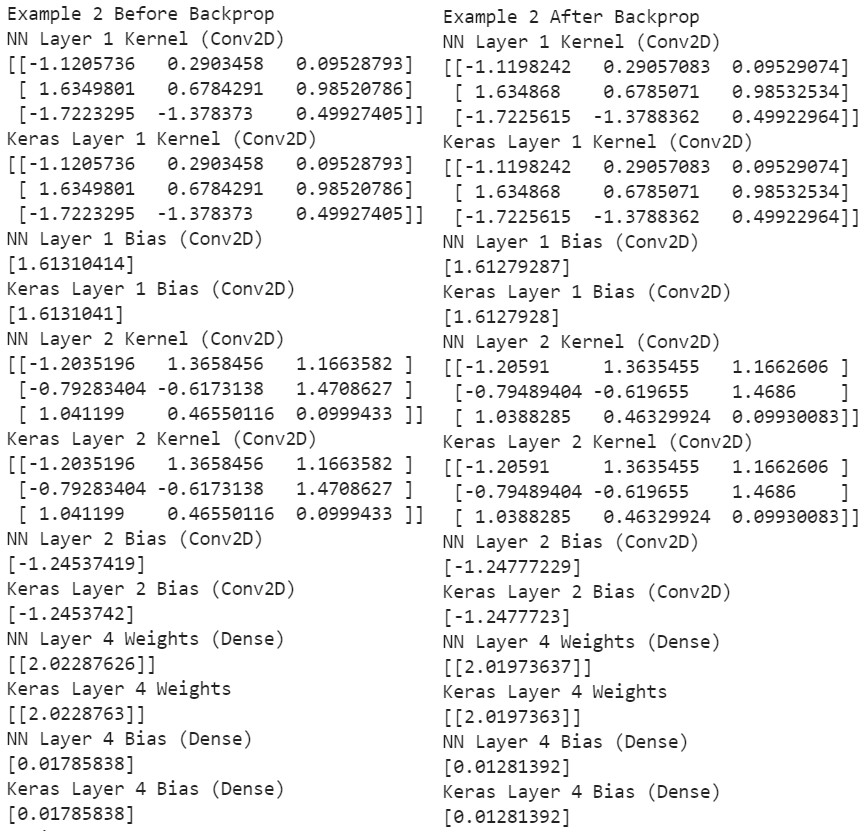
\includegraphics[width=\linewidth]{example-2-weights.png}
  \caption{Weight comparison for example 2.}
  \label{fig:e2}
\end{figure}

\begin{figure}
  \centering
  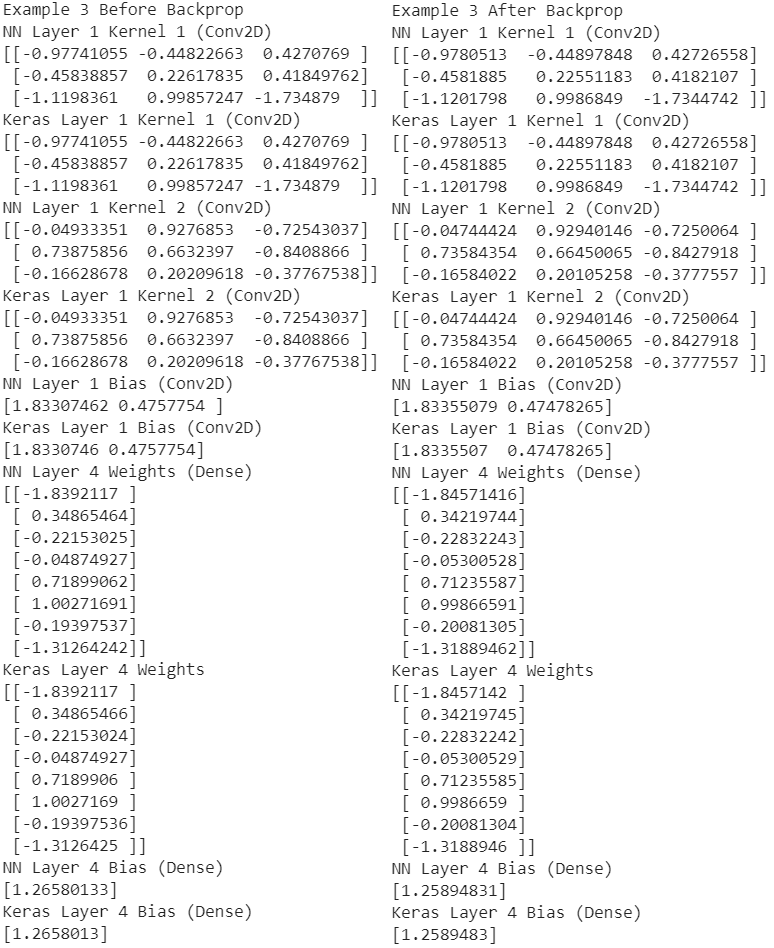
\includegraphics[width=\linewidth]{example-3-weights.png}
  \caption{Weight comparison for example 3.}
  \label{fig:e3}
\end{figure}

\bibliographystyle{abbrv}

\end{document}